\documentclass[varwidth=true, border=2pt]{standalone}

\usepackage{pgfplots}
\usepackage{tikz}

\usetikzlibrary{calc,patterns,angles,quotes}

\begin{document}
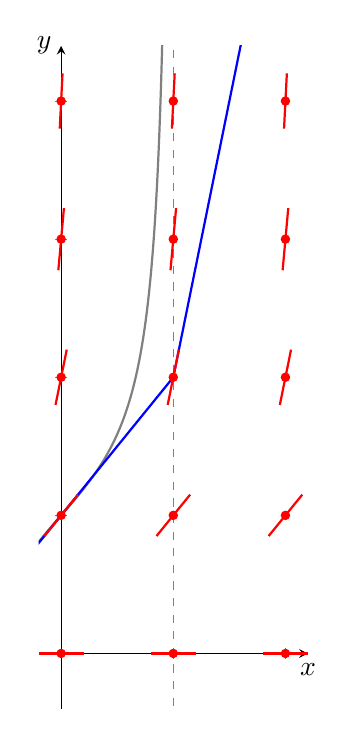
\begin{tikzpicture}
    \begin{axis}[
        legend pos=south east,
        axis x line=middle,
        axis y line=middle,
	every axis x label/.style={at={(current axis.right of origin)},anchor=north},
	every axis y label/.style={at={(current axis.above origin)},anchor=east},
	xticklabels=\empty,
	yticklabels=\empty
        grid = none ,
        width=5cm,
        height=10cm,
        grid style={dashed, gray!1},
        xmin=0,     % start the diagram at this x-coordinate
        xmax=2,    % end   the diagram at this x-coordinate
        ymin=0,     % start the diagram at this y-coordinate
        ymax=4,   % end   the diagram at this y-coordinate
        xlabel=$x$,
        ylabel=$y$,
        enlargelimits=true,
        tension=0.08]

         \addplot[domain=-4:4, blue,samples=250] {-x-1};
         \addplot[domain=-0.2:1, gray,samples=250, thick] {0.6*tan(deg(1.55*x))+1};
         \addplot[dashed,gray,mark=none] coordinates{(1,-0.5)(1,5)} node[below, pos=0] {};
         

 	 \addplot[domain=-1:1, blue, thick,samples=250] {x+1};
 	 \addplot[domain=1:2, blue, thick,samples=250] {4*x-2}; 

	\addplot[domain=-0.2:0.2, red, thick]{0};
	\addplot[domain=0.8:1.2, red, thick]{0};
	\addplot[domain=1.8:2.2, red, thick]{0};
	\addplot[domain=-0.15:0.15, red, thick]{x+1};
	\addplot[domain=0.85:1.15, red, thick]{x};
	\addplot[domain=1.85:2.15, red, thick]{x-1};

	\addplot[domain=-0.05:0.05, red, thick]{4*x+2};
	\addplot[domain=0.95:1.05, red, thick]{4*x-2};
	\addplot[domain=1.95:2.05, red, thick]{4*x-6};
	
	\addplot[domain=-0.025:0.025, red, thick]{9*x+3};
	\addplot[domain=0.975:1.025, red, thick]{9*x-6};
	\addplot[domain=1.975:2.025, red, thick]{9*x-15};

	\addplot[domain=-0.0125:0.0125, red, thick]{16*x+4};
	\addplot[domain=0.9875:1.0125, red, thick]{16*x-12};
	\addplot[domain=1.9875:2.0125, red, thick]{16*x-28};

	\addplot[red, only marks, mark=*, mark size=1.5pt] coordinates{
	(0,4)(1,4)(2,4)
	(0,3)(1,3)(2,3)
	(0,2)(1,2)(2,2)
	(0,1)(1,1)(2,1)
	(0,0)(1,0)(2,0)
	};
	

    \end{axis}
\end{tikzpicture}
\end{document}